Ting fra discussion jeg har flytta:
\section{ClickHouse}

% Originally scenario 2
Resistance to deletion

In summary, both backup types were resistant to deleted or encrypted backups. 
The soft delete functionality in Azure is very powerful, and along with monitoring systems in Azure that notifies both when backups are deleted and when soft-delete is disabled, it is not likely that such an attack would go unnoticed either. 

Since Azure Backup stores read-only snapshots of the VM,
which cannot be changed, we find it unlikely that an attacker would be able to encrypt Azure Backup's backups directly.
The possibility of corrupting backups by overwriting them with encrypted database data was explored in scenario 1,
where we concluded that it would be unlikely.

By using soft delete, it is possible to recover deleted backups made with both Azure Backup and clickhouse-backup.
Soft delete is enabled by default for Azure Backup,
but has to be enabled manually for the Storage Blobs used by clickhouse-backup.
Enabling it is not particularly difficult, though.
As long as soft delete remains enabled, we believe both backup solutions can recover from attempts at deleting the backups.
As we will see in scenario 3, though, soft delete can be disabled,
which means backups can be permanently deleted. Soft delete alone is not sufficient.



\subsection{Resistance to ransomware [TODO]}

Azure Backup's backups are read-only, which means they can't be overwritten.

The same is true for 
Azure Blob Storage, which is one of the supported remote storage solutions for clickhouse-backup,
support 

\subsection{Performance [TODO]}
% Discussion
%The time it takes to rebuild the environment can vary greatly.
%If IaC is used, one can expect the time to be quite short, for example.
%We will therefore be measuring the time it takes to get the database fully operational again.





\subsection{Ease of use [TODO]}

\subsubsection{Azure Backup}

We found Azure Backup is easy to set up.
It can be configured with the Azure Portal,
which is good for learning the system and discovering features.
Azure Backup uses "Backup Policies" to configure backup routines.
These policies define how often backups should be made,
how long they should be retained,
the type of encryption to use,
the data redundancy tiers, and more.
A policy can be defined once and applied to multiple VMs.
This makes it easy to achieve compliance with the organization's backup policies.

\subsubsection{clickhouse-backup}

We found clickhouse-backup to require more manual configuration than Azure Backup does,
in order to achieve an equivalent setup.
A yaml file is used to configure options like remote storage.
The configuration file stores informat10:02:43.087969ion %hva skjer her
like access keys and SAS tokens,
which are used to provide access to resources.
Though the type of access can be limited when generating the SAS token,
care must be taken to ensure that this information is not leaked.

When clickhouse-backup fails,
the error messages can be difficult to interpret,
making troubleshooting difficult.
When we were working on performance tests for ClickHouse,
we had trouble downloading the remote backups (see \ref{app:chbk-perf} for details).

Troubleshooting obscure error messages is the last thing you want to do in an emergency.

\subsection{General discussion [TODO]}

Azure Backup is more flexible than clickhouse-backup,
in the sense that it can be used to backup a greater number of services.
clickhouse-backup can only back up ClickHouse databases.
Azure Backup can back up any VM, and can also backup various Azure services.
This makes it ideal for organizations that are already invested in the Azure ecosystem.

clickhouse-backup is not tied to any single cloud environment.
Instead, it supports multiple environments and storage types.

\subsection{From ch6}
After a holistic analysis of the backup solutions we explored for ClickHouse,
we have concluded that Azure Backup is the option we would recommend.
Azure Backup is easy to use and maintain,
provides a number of security features.

MUA can greatly increase resilience against attacks against backups,
as it prevents privileged actions without the confirmation of another, specific account.
In a human-operated ransomware attack, 
the attacker would need to 

Azure Backup is generally more expensive than clickhouse-backup using Storage Blobs.
Depending on how valuable the data is, 
This may be 
But still not prohibitively expensive.
This all depends on how valuable the data is of course.

Issues when recovering clickhouse-backup.
Generally difficult to troubleshoot.
More configuration required.

Azure Backup has excellent performance as long as an Instant Restore point is available.
The number of Instant Restore points affect cost.


Integrates well with other Azure services.
Should be quite easy to 

Azure is quite business oriented.
Easy to achieve compliance with policies.





\section{PostgreSQL}
The overall process of backing up and restoring a managed PostgreSQL instance in Azure left us impressed with the ease of use and efficiency of the processes. This proves to be the case with both Point-in-time Restore (PITR) and Azure backup with Backup vault. Despite this, neither solution was the complete package and some major configuration was required to bring especially the Azure backup-solution up to a satisfying standard. Several important and effective security features were completely lacking as well, and future updates of Azure Backup for PostgreSQL should address these. 

\subsection{Resistance to Ransomware}
On of the primary criteria for the analysis in this project was to determine whether the chosen backup solutions were able to protect against data loss in the event of a ransomware attack. Our tested solutions for Postgres were able to meet this requirement, but neither of the two solutions were sufficient on their own. PITR supports restoring data even if deleted, and withstood all of our scenarios in terms of ransomware protection. 

The lengthier retention of Azure Backup was however missed in PITR. With human operated ransomware it's not impossible that the data in the database is bad data even long before the organisation notices something is wrong. Azure backup however lacks several important security features, such as soft-delete and MUA in its implementation for Postges databases, so it alone is not secure enough if an attacker has gained enough access to the organisations systems. The possibility of separation of duties (and privileges) made possible by the backup being a completely different resource, able to be managed by a completely different administrator was also a big advantage.  

%Ability to recover encrypted files
%• Resistance to ransomware spread.
%• Ransomware detection.
%21
%Chapter 3: Method 22
%• Ability for backup to withstand encryption
%• Ability for backup to withstand deletion

\subsection{Performance}
The difference in recovery time between PITR and Backup vault is significant, but does not exclude the use of one or the other, as they have different functions. PITR provides more fine-grained control of the exact recovery point, where backup vault only saves the state of the database as often as defined in the backup policy. In return, backup vault provides the opportunity to recover to a point far back in time, up to 10 years, where PITR only has an approximate maximum of a month back in time.

%\subsubsection{Performance future work}
%\paragraph{Infrastructure Double encryption effect:}
%Measure whether there is a noticable difference with and without the use of infrasctructure double encryption feature when creating the server. To avoid expected margin of error the database should be scaled up to 40 GB.

%\paragraph{Flexible server, being burstable effect on restore time}
%Again with scaled up databases (40 GB), test out whether having a burstable flexible server affects restore time where adding to vCores when restoring will decrease the restoration time compared to operating on the normal amount used in a general purpose single server.

\subsection{Cost}
The cost of the backup solutions proved not to be as great a consideration as we initially assumed it would be. This is due to the cost of a PostgreSQL single server managed database depending greatly on the server configuration rather than the backup architecture solution. 


\subsection{Ease of use}
Both backup solutions tested proved in general to be easy to use, so much so that we felt we became quite proficient through the course of our experiments. There were complexities to work through, and additional configurations that required more effort than we would have liked -- especially for the Azure Backup-implementation. 

Setting up PITR was about as easy as it could possibly be, as it was a built-in feature of the Postgres database instance. Azure Backup needed a little more work, but clear documentation and simple wizards caused this to also be quite trivial. 

Setting up the alert rules were however far more cumbersome than we would have liked. Despite the appendixes of this report showing the simple solution once we found it, it took more time than we would have preferred. The frustration lies not as much with the process itself, but the fact that there is very little in the Azure documentation to serve as a guide when undergoing the process. The alerts we had to set up manually were of course expected to be turned on by default, and as such there was no documentation that showed how to do it manually. This was a strenuous and unnecessary part of the setup process, and as it so closely ties to good security practices, it should not be that difficult. Some administrators will surely discover the same problem as we did, but not bother to fix it simply because they can not presume that the return on their time investment is worthwhile.

%Bytt tilbake hvis ønskelig :)
%Some administrators will surely discover the same problem as we did, but not bother to fix it, simply because humans are humans, and there is often not enough time to do a thorough job. 

The recovery process was simple enough for both solutions, but needed the setup and configuration of new server instances. This didn't make the process much harder however, and it is probably safest to setup a new server instance anyway, in case the attackers have installed some backdoor to return later. The process should ideally be scripted or be automated in some way to maximise RTO, and minimize risk of human error. 

Both solutions offered the ability to regularly test the backup instances manually, as restoring to a backup does not need to interfere with the production environment what so ever. This makes it possible for administrators to manually (or automatically) monitor the automatic backup solution in the organisation to check that they are still protected. Regularly testing disaster recovery solutions is an important part of the protection efforts, so this is a welcome possibility.  

\subsection{General discussion [TODO]}

The initial goal was to protect a managed Postgres instance with the different backup solutions we figured would be most effective in protecting it. The two chosen were initially meant to be compared and then one of them selected as the superior solution based on whichever needs an organisation might have. What we have discovered through our experiments and research however is that they are perfect complements to one another. PITR and Azure backup for Postgres are both decent solutions, but the strengths of one fills the weakness of the other, and vice versa.

In general 

\subsection{PostgreSQL (from ch6)}


The deciding factor for cost was the amount of vCores and size of RAM. In short, virtual Cores, or rather vCores, are a simplification that make it easier to translate the hardware spec needs of an on-prem infrastrucure into one hosted in the cloud.

In our experiments we used a 4vCore 100 GB server in the General purpose tier. General purpose is well suited for the hosting requirements of an average organisation. The step up from general purpose tier would be memory-optimized, which provides faster transaction processing and higher concurrency. We can also assume a better recovery time for the memory-optimized servers though we did not conduct performance tests to confirm our belief. The guidelines set by Azure steered most use cases into the general purpose tier, which is where our experiments set their focus. The price of a General purpose, fifth generation, 4vCore, 100GB server was approximately 260 US Dollars a month [CITE]. %cite https://azure.microsoft.com/en-us/pricing/details/backup/
The backup solution pricing depends greatly on the form of archiving, where locally-redundant is half the price of geo-redundant storage. In a holistic sense determining the cost factor is not useful since Azure has the ability to cater to the specific needs of an organisation in such a way that an identical service architecture can vary greatly in cost depending on miniscule details in configuration.

However, one general recommendation relating is the use of linux-based flexible server instead of the windows-based single server for managed PostgreSQL. It provides several features such as being able to scale up or down in tier according to load, schedule maintenance windows as well as the ability to temporarily stop the server, among other cost-saving features.


\section{Drøft løsning}

[Note: Liker ikke helt dette som er skrevet/måten det er skrevet på... Virker litt ufokusert. Kan heller bare foreslå løsningen rett i konklusjonen mener jeg.... ]

Based on the results of our tests and the theoretical background these tests were based on, we propose the following recommendation for a backup solution using Azure Backup. This solution is not a complete system architecture, as that would be beyond our scope, but simply the features we deem necessary to minimize the risk of data loss because of ransomware. 

Azure Backup must be configured with policy settings according to each organisations needs. For data that rarely changes, but which is business critical, the frequency of backups could be lower whilst the redundancy is higher. On the other hand, for data that is less critical, but often updated, frequent backups may be handy, whilst the regular redundancy tiers may be enough. This is for each organisation to decide based on their needs and budget. 

Ensuring the most important security features of Azure Backup are enabled is however necessary no matter what type of data is backed up. Soft-delete is enabled on all recovery service vaults by default. To further ensure the security of backups, multi user authentication ought to be enabled on all recovery service vaults in an organisation in order to prevent unauthorized disabling of soft-delete or deletion of backups. Using multi user authentication demands that the organisation also has tight control over their domain, and effectively use role based access control to control access. In a zero trust environment with just-in-time access to both performing destructive actions, and approving them, the chance of an attacker managing to tamper with the backups is significantly reduced.  




\subsection{Research questions [TODO]}

\subsection{Security aspects beyond our scope}
%Er det verdt å skrive om det som er utenfor vårt scope? Hjelper for å sette i kontekst, men skal vi det?

Despite the security features of Azure working as expected, and our own inability to permanently compromise our data within the scope of our scenarioes, there is no doubt that more has to be done. As the time spent performing the analysis testifies to, nothing is ever easy if you do not do it often. As with the principles of Infrastructure as Code from chapter  \ref{IaC}, you cannot expect to handle a disaster if you never practice it. Designing the infrastructure that the backup solution lives in to handle unexpected downtime, outtages, data loss, and worse is essential to managing to restore in a reasonable amount of time. 

Culture, Security culture




\chapter{Scenarios}
[Mye av dette skal flyttes til kapittel 3, men vi vil vite at ting legges inn skikkelig.]

\section{Ransomware encrypting files on a Clickhouse server randomly}

\subsection{Conditions}

\begin{itemize}
    \item Access to the server (able to execute programs remotely, ssh, etc.)
    \item Permissions on the server, in order to overwrite restricted files.
\end{itemize}

\subsection{Etc}

In order to avoid breaking the victim's system,
ransomware often uses a whitelist of directories and file extensions to determine which files to encrypt.
If the system were to be broken, the  victim would be unable interact with their computer,
and [...]

Whether Clickhouse files would be affected depends on the whitelist used.
Clickhouse stores data in [INSERT FILE/DIRECTORY] by default. 

If the ransomware were to encrypt a Clickhouse database file, [...]


\section{Multi-user authentication for backup and subscription deletion}
\subsection{Conditions}


\subsection{Consequences}

lorem ipsum

\subsection{}

\section{Dead Ends}

\subsection{Testing whether resource migration can allow for key vault purge protection to be turned off}
To test this out an Azure Database for PostgreSQL Single Server was set up, along with the corresponding key vault. Purge protection was turned on when creating the key-vault, which enforces a mandatory retention period where there is no way to delete the key vault or turn off the purge protection. The key vault holds a connection string to the database, and the goal is to make this inaccessible. Azure has an option to migrate a resource to another resource group. 

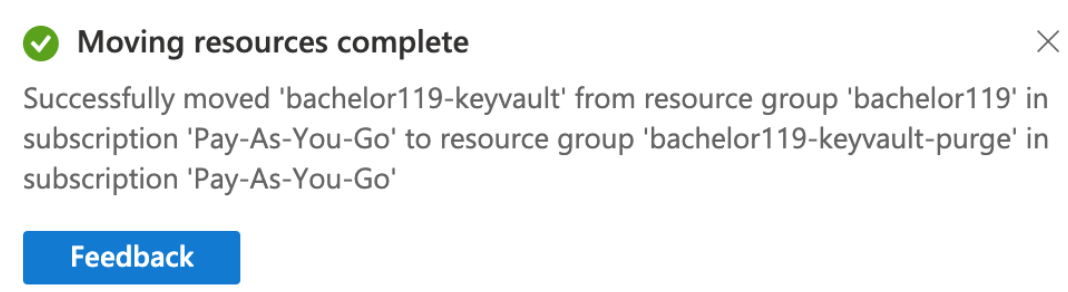
\includegraphics[scale=0.5]{figures/migrate-resource-success.png}

Now it would be interesting to find out what happens when migrating the key vault to a resource group and deleting said group. Testing this out by deleting the resource resource group and the key vault:

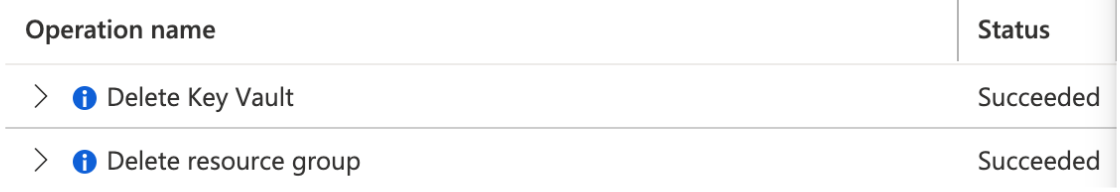
\includegraphics[scale=0.5]{figures/delete-group.png}

Managing deleted key vaults allows the recovery of the key vault. This actions also recreates the previously deleted resource group.

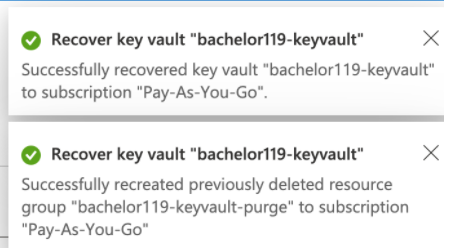
\includegraphics[scale=1.3]{figures/recover-vault.png}

This establishes that purge protection is a safe mechanism for ensuring key vaults regardless of resource group environment. It can not be deleted before the retention period has passed.

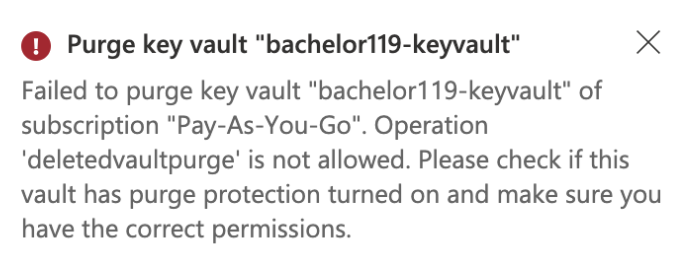
\includegraphics[scale=.8]{figures/purge-denied.png}

It is worth noting that attempting the resource migration and deletion action on a backup vault will not work. In this case the backup vault can not be deleted since it has an active instance being backed up. 

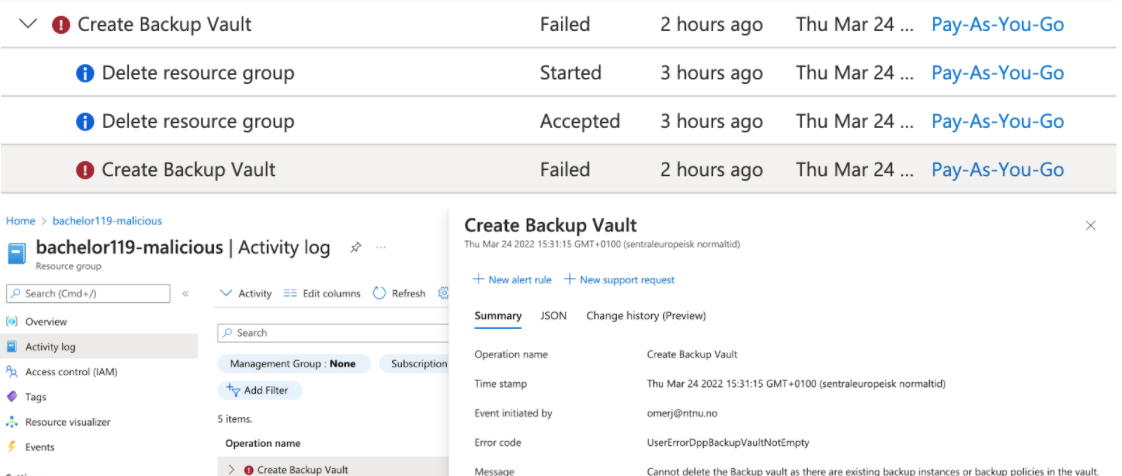
\includegraphics[scale=.7]{figures/backup-migration.png}

\subsection{Deleting a backup vault}
%Worth looking into resource guard here
To delete a resource group with a backup vault:
\begin{enumerate}
    \item Suspend backups of backup instance
    \item Delete backup instance
    \item Delete backup policy
    \item Delete backup vault
    \item Delete resource group
\end{enumerate}
 Each step is is a prerequisite for the next one. You can not delete a backup instance if it is in use, meaning not suspended. You can not delete a backup policy if there is an instance using that policy. The same goes for policy in vault and vault in resource group.

% Backup vault for a postgreSQL flexible server. Set up with data
% Set up policy. Delete database and restore from backup. Record time it takes.
% 

% Can you somehow delete all backups as well?
% Test the same with resource guard.
%
%TODO first thing: Migrate data.

%flexible can restore to a different Vnet while single can only restore to the same one.

%Can you use backup vault for Azure Database for PostgreSQL single server?

%If not, what options are there?

%Test out option. Compare to flexible server restore time.

%Should I add a read replica for PostgreSQL single server?
%write a bit about different ways of backing uup
%https://www.postgresql.org/docs/current/backup.html#:~:text=There%20are%20three%20fundamentally%20different,Continuous%20archiving

\section{Multi-User Authenication takeover}
Unlikely?
Requires 2 specific accounts.
